\section{Evaluation}
\label{sec:evaluation}
DCG-UPUP-Away is evaluated in two experiments.
First, a simulated turtlebot within randomly generated simulated environments is given a series of user-generated natural language commands.
Second, a physical turtlebot is given specific commands in a laboratory environment in order to demonstrate novel behaviors enabled by DCG-UPUP-Away.
Both experiments assume a perfect object recognizer that translates raw sensor data into a world model $\Upsilon$ that may be used by DCG-UPUP-Away, as well as an initial set of hand-labeled training examples for training the LLM to ground cubes, spheres, and cylinders.
In all trials, training DCG-UPUP-Away with 53 positive examples took less than 1 minute on a Lenovo Thinkpad X1 Carbon (TODO get more specs), and grounding a command took under 40 seconds.\\
\subsection{Experimental Setup}
\indent The simulated testing environments are randomly generated in Gazebo.
10 worlds are created, and each is populated with a random collection of objects in randomized locations.
There are 8 possible object types (including cubes, spheres, and cylinders) in 3 possible colors, for a total of 24 objects.
Each object has a 15\% chance of being added to a given map.
Using such a procedure to generate environments, when coupled with the limited field of view of the turtlebot, caused 87\% of objects to be placed outside the initial field of view of the robot, demonstrating the need for the ability to ground commands to hypothesized objects.\\
\indent After generating the 10 maps, screenshots of world with a single object highlighted are uploaded to Amazon Mechanical Turk.
For each image, users were instructed to write a command ``for approaching the highlighted object.''
These image-command pairs were saved for evaluating whether a robot, when placed in the corresponding simulated world and given the natural language command, successfully approaches the correct object.
An example screenshot, with an annotation supplied by a user, is shown in Figure~\ref{fig:amt}.\\
\begin{figure}[h]
	\centering
    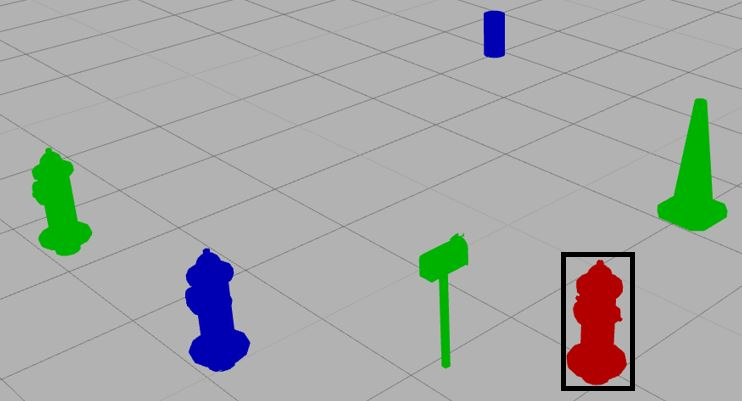
\includegraphics[width=8.5cm]{amt}
	\caption{A simulated world with a highlighted object presented on Amazon Mechanical Turk, labeled by a user as ``Move to the red fire hydrant.''}
	\label{fig:amt}
\end{figure}

\indent 10 image-command pairs are randomly selected without replacement from the pool of all pairs.
The 10 ordered pairs constitute one trial; each specific pair is dubbed one iteration.
30 trials are generated, each consisting of 10 iterations, for a total of 300 evaluations.
When executing a trial, the turtlebot is first trained on the initial, hand-curated training set.
The turtlebot is then given the natural language command from the first iteration, and then retrained using the initial data supplemented by unsupervised training examples generated by the first iteration.
The retrained turtlebot is given the command from the next iteration, and appropriately retrained after each execution until all 10 iterations have been executed.\\
\indent The metrics we consider are the grounding accuracy (how likely DCG-UPUP-Away is to correctly ground a phrase) and the number of known symbols.
We further divide the grounding accuracy results to examine when phrases are grounded to known, unknown, or learned objects.
\subsection{Grounding Accuracy}
The primary metric used in evaluating the success of DCG-UPUP-Away is the grounding accuracy: how likely is the turtlebot to correctly execute the natural language command.
Because the turtlebot is retrained between iterations, grounding accuracy may change as a function of iteration number.
In fact, mean grounding accuracy remains between 70\% and 90\% across all iterations, as shown in Figure~\ref{fig:g_acc}.\\
\begin{figure}[h]
\centering
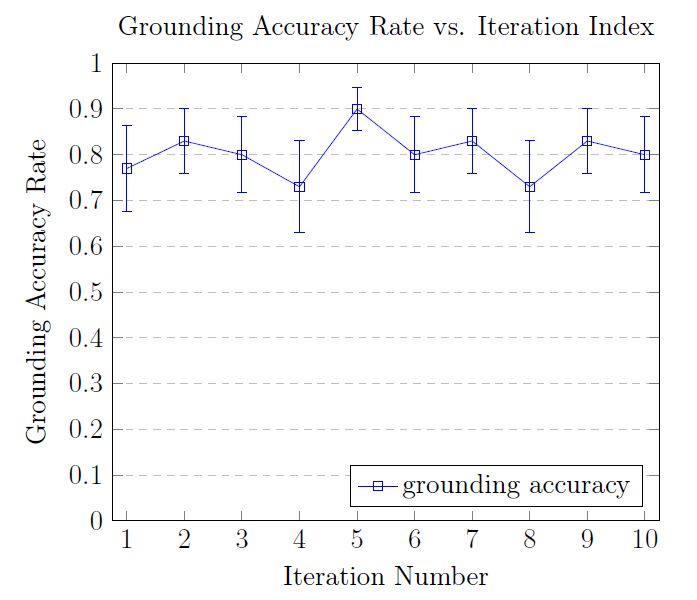
\includegraphics[width=8.5cm]{g_acc}
\caption{this is the overall grounding accuracy}
\label{fig:g_acc}
\end{figure}

\indent Although the overall grounding accuracy remains relatively constant, the underlying behavior within DCG-UPUP-Away changes over the course of a trial.
In Figure~\ref{fig:g_acc_split}, we plot 3 curves, showing what fraction of correctly grounded phrases refer to known objects, unknown objects, or learned objects as a function of iteration number.
In the first iteration, nearly 70\% of correctly grounded commands refer to known objects, but by the 10$^\text{th}$ iteration that number has fallen to nearly 10\%, replaced almost entirely by correctly grounding to learned objects.

\begin{figure}[h]
\centering
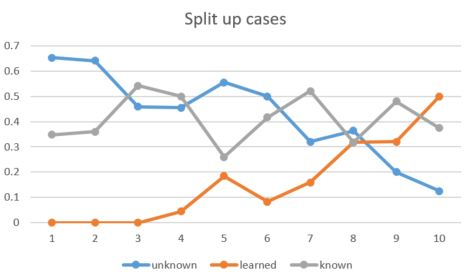
\includegraphics[width=8.5cm]{learning}
\caption{this is split up (must replot well)}
\label{fig:g_acc_split}
\end{figure}


\subsection{Learned Symbols}
In order to better examine the learning behavior exhibited by DCG-UPUP-Away, the other metric considered is the number of correctly known symbols.
(Symbols may be incorrectly learned by associating a phrase with the wrong sort of object.)
Initially, the turtlebot is trained with cubes, spheres, and cylinders, but environments may contain up to 5 additional object types (fire hydrants, drills, mailboxes, door handles, and traffic cones).
Whenever an unknown phrase is grounded to such an unknown object, the turtlebot learns the new symbol.
Thus, one may calculate the expected number of known symbols as a function of iteration number using combinatorics to count how many unknown objects are present.
The recorded number of correctly learned symbols are plotted in Figure~\ref{fig:symbols} in blue, as well as the expected number in red.\\
\begin{figure}[h]
\centering
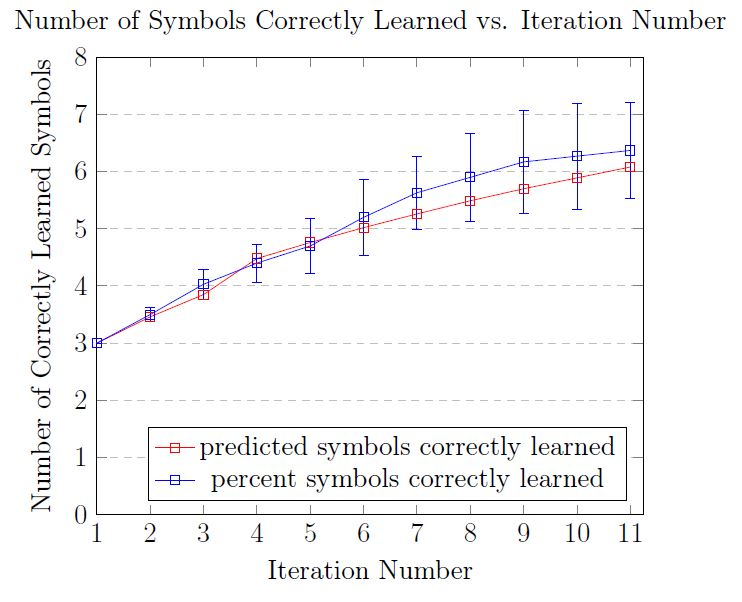
\includegraphics[width=8.5cm]{symbols_corr}
\caption{this is how we show that we learn symbols. I will update this label (and caption) of this figure. also must use std error bars instead of variance}
\label{fig:symbols}
\end{figure}
(Asking for advice: the x axis ranges from 1 to 11 because I can retrain after the 10th iteration and increase the mean number of symbols learned. It's a small increase, though, so I wouldn't be too upset cutting off the 11th iteration, though.)

As expected, the blue curve starts at 3 (for the cube, sphere, and cylinder), and stochastically monotonically increases.
In 10\% of trials, all 8 symbols were correctly learned; in other trials DCG-UPUP-Away incorrectly grounded unknown phrases (and therefore learned an incorrect symbol) or the 10 iterations collectively never referred to the five initially unknown objects, preventing DCG-UPUP-Away from ever learning the new symbol.
Furthermore, learning symbols correctly improves grounding accuracy: for each additional correctly learned symbol, the turtlebot is over 4\% more likely to correctly ground a command. (TODO generate p values via ANOVA.)

\subsection{Hardware Demonstration}
Outside the simulation environment, DCG-UPUP-Away was tested on a physical turtlebot in a laboratory setting.
The turtlebot was placed facing a cylinder (known) and a cone (unknown).
In addition, a cube (known) and a crate (unknown) were located behind the turtlebot.
All objects were labeled with AR-track tags, which, in conjunction with (cite AR track package) was used in order to generate the world model $\Upsilon$ from a kinect mounted on the turtlebot.\\
%I'd like to add a footnote saying that I have videos of these demos
\indent Four natural language commands were used to demonstrate the full range of abilities of DCG-UPUP-Away.
First, the turtlebot was given the command ``move towards the cube.''
The turtlebot successfully drove to the cube, demonstrating a correct grounding to a known, perceived object.\\
\indent Second, the turtlebot was given the command ``move towards the cone.''
The turtlebot drove to the cone, demonstrating that it perceived the cone as unknown, recognized the phrase ``cone'' as unknown, and grounded the unknown phrase to the unknown object.
Thus, a command was correctly grounded to an unknown, perceived object.\\
\indent Third, the turtlebot was given the command ``move towards the cube.''
The turtlebot rotated in place until the cube came in view, and then approached the cube.
In other words, the command was first grounded to a known, hypothesized object and then, once then cube was perceived, to a known, perceived object.\\
\indent Fourth, the turtlebot was given the command ``move towards the crate.''
Once again, the turtlebot rotated in place, this time until it saw the crate, whereupon it drove to the crate.
This demonstrates two important behaviors: 1) the turtlebot must have learned what a cone was, otherwise the unknown phrase (``crate'') would have been grounded to the cone and 2) the turtlebot grounded the command to an unknown, hypothesized object until the crate was perceived.
The execution of this last command, including images of the physical behavior of the turtlebot as well as the model used for grounding, is shown in Figure~\ref{fig:hardware_demo}.

\begin{figure}[ht]
\centering
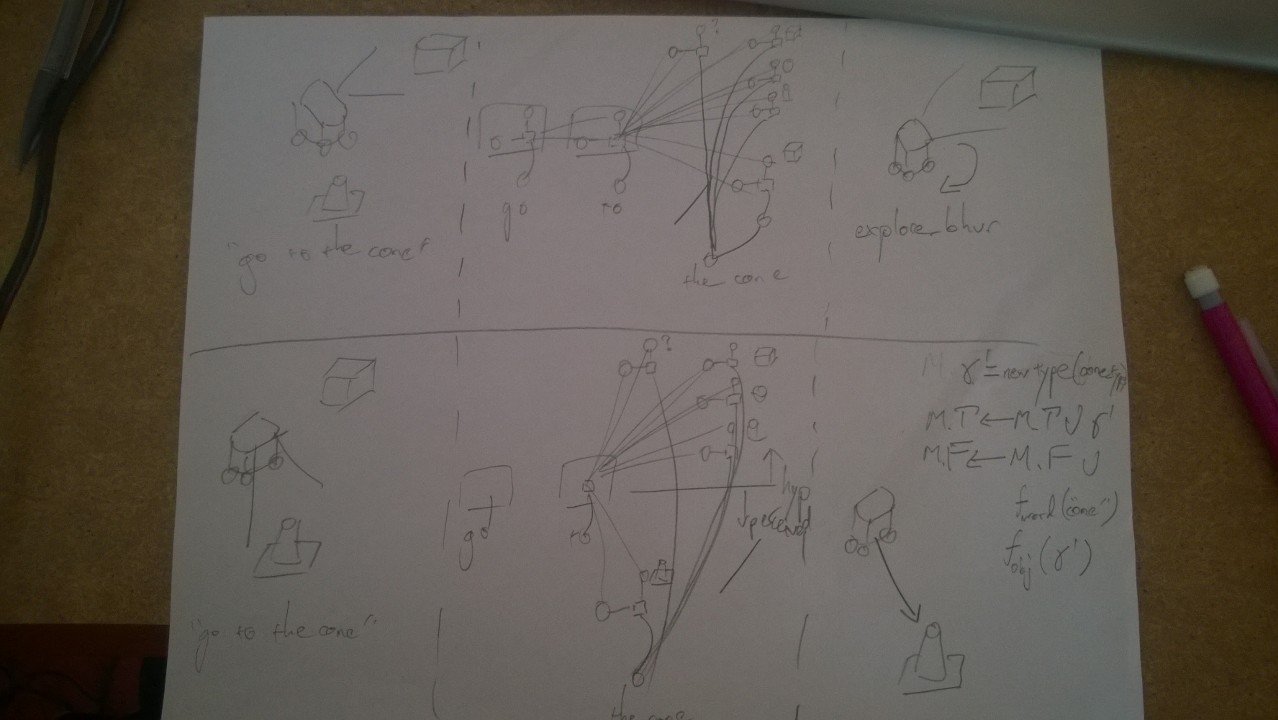
\includegraphics[width=8.5cm]{hardware_sketch}
\caption{this is a sketch of the 6 subfigures that demonstrate hypothesized groundings on hardware and in the model, and shows how it learns. I'd like this to go across the top of the page.}
\label{fig:hardware_demo}
\end{figure}

\subsection{Limitations}
Although the successful execution of natural language commands has been discussed in great depth, the failures of DCG-UPUP-Away are equally important in characterizing the limits of its performance.\\
\indent Specifically, the most obvious limitation is that DCG-UPUP-Away assumes that, in the absence of additional information, unknown phrases refer to the first perceived unknown object.
Strategies to relax this assumption by associating language adjectives with object properties have been explored in Section (TODO color section), but so far only a relatively simple method has been used.\\
\indent In addition, DCG-UPUP-Away assumes a one-to-one correspondence between unknown phrases and unknown objects; it cannot, for example, learn synonyms by grounding unknown phrases to known types.